\section{System Overview}
\label{sec:overview}

\hyphenation{com-mit-ted}

% Distributed DB
Mediator operates on top of a distributed key-value store with a
{\em get\/}/{\em put\/} API that provides a read/write access to data items identified by unique keys. For scalability, 
the data can be partitioned over multiple nodes. In this context, all accesses 
to a given item are served by a single node ({\em database server}). The get/put
API is called {\em native}, in contrast with Mediator's API that is {\em transactional}. The database
serves both types of traffic. Native clients are unaware of concurrent transactions. 

Mediator assumes 
multi-version concurrency control~\cite{GrayTP1993} in the underlying database.
Namely, every update creates a new version of the data item, and multiple versions 
can be accessed in parallel. The transaction processor maintains a global logical clock 
to timestamp all transactional writes. The execution is optimistic -- i.e., each transaction
runs unobstructed until commit, whereupon consistency is enforced. At that point, 
semantic conflicts are detected through version timestamps, and the compromised 
transactions are aborted. 

Mediator shares many design principles with Omid~\cite{Omid2014}. Similarly to
Omid, Mediator employs a  standalone {\em transaction status oracle} service (TSO), which maintains the clock and tracks the state required for guaranteeing the safety
properties.  Transactional clients use this context to read the correct data versions 
and to timestamp their writes. A transaction communicates with the TSO twice -- upon begin, 
to retrieve the required state, and upon commit, to resolve the conflicts with the concurrent 
transactions. The key for scalability is keeping the TSO separate from the datapath.

% TSO scalability
The TSO is highly optimized, to prevent it from becoming the system's bottleneck. 
A transaction starts getting tracked only once it issues a commit request. A client
communicates to the oracle the set of keys accessed by the transaction.
The Mediator TSO stores it in a compressed Bloom filter~\cite{Bloom1970} form,
hence each transaction's footprint is fixed and small.  Mediator adopts Omid's 
optimization of replicating the oracle's state to the client upon transaction begin,
to enable local decision-making~\cite{Omid2014}. For clients with persistent TSO 
connections, this replication is incremental and efficient.

\remove{
% Clock propagation
Guaranteeing a logical order between transactions and native operations 
requires some coordination of the local database server clocks with the global clock. 
For this, Mediator clients piggyback the global clock's value retrieved from the TSO 
on top of the datapath requests served by the database (Section~\ref{sec:algorithm}). 
The oracle does not communicate with the database directly, to avoid becoming a bottleneck. 
}
% Deferred updates 
%In rare cases when transactions get aborted, their changes are rolled back. 
In multi-version databases, concurrent transactions are protected 
from reading non-committed writes by creating new versions with timestamps
that are beyond the read horizon. This approach is non-applicable 
in our setting, since native reads that simply retrieve the latest data versions 
must be protected. Instead, Mediator clients buffer the updates locally, and write them 
back upon commit. Prior to updating the database, the client atomically appends its 
modification set to the write-ahead log (WAL).
This is in contrast to other transaction processor
implementations~\cite{Percolator2010,Omid2014} writing eagerly to the database.
These implementations exploit the durability of database updates and therefore
avoid managing a separate log.
Mediator's performance for the {\em transactional\/} 
part of the traffic is therefore a-priori inferior to eager-write systems. 
Section~\ref{sec:algorithm} describes the optimizations that target this gap.

% Recovery
Since Mediator's writes are deferred until commit, it never needs to roll back aborted 
transactions. However, a failure of either a client or a database server in the middle 
of a distributed write-back can leave transactions--that are committed in the
log--incomplete.
While the algorithm guarantees that subsequent transactions always observe 
a consistent database state, some of them might get blocked and eventually
abort due to dependencies on incomplete transactions. To guarantee progress, 
the TSO helps uncompleted transactions finish their database update. It
periodically initiates a helper process that locates their commit records in the log, and replays 
them in an idempotent way~\cite{GrayTP1993}. Transactions that failed to log their
changes prior to the helper's execution are 
%cut off by setting a low watermark on 
%the commit timestamp. Hence, they effectively 
(possibly spuriously) aborted. 

\begin{figure}

\centering {
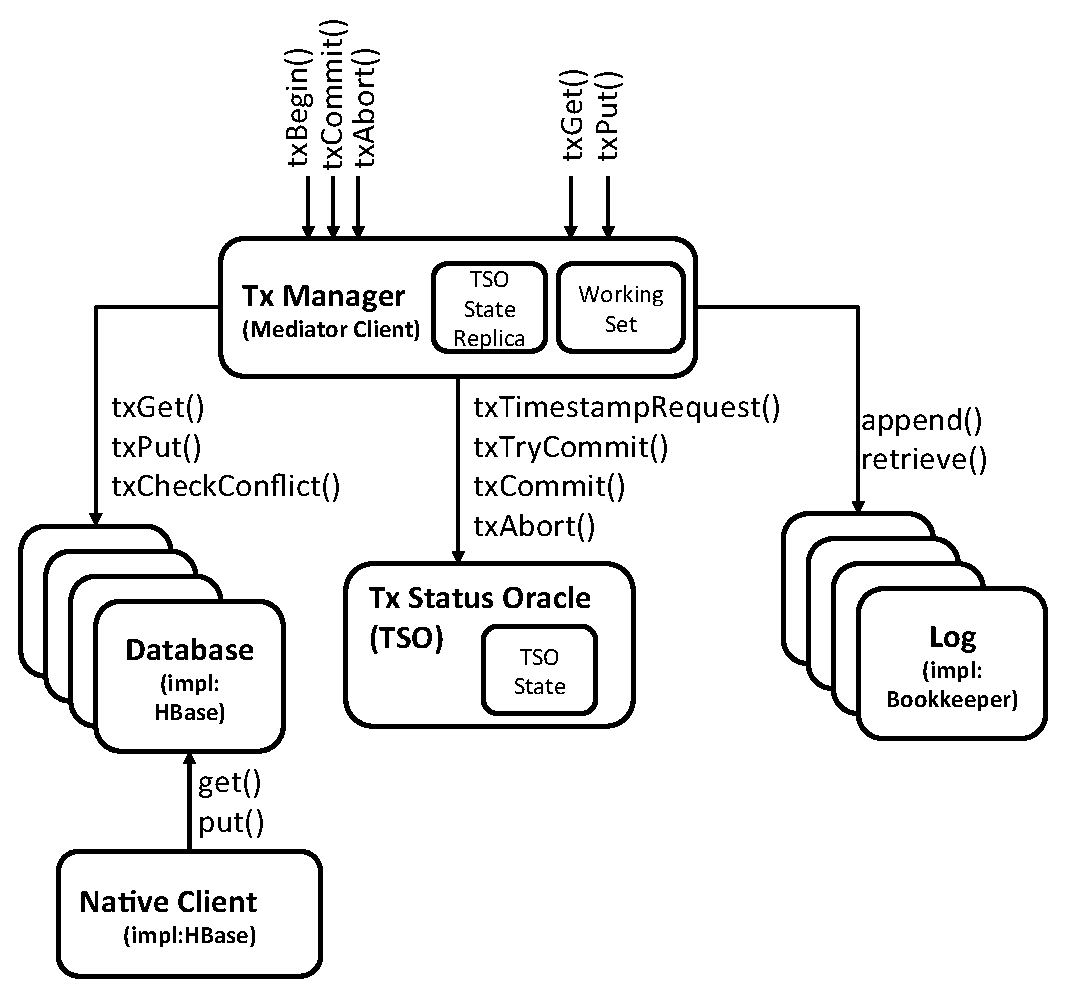
\includegraphics[width=3in,clip]{Figs/mediator_arch.eps}
}

\caption{\bf{\small{Mediator architecture. The transaction manager (Mediator client)
employs three backend services -- the database, the log, and the transaction status oracle (TSO). 
The database serves native clients directly, and provides Mediator clients with a backdoor API. 
}}}
\label{fig:mediator_arch}
\end{figure}
 
Oracle's failures are handled similarly. Upon recovery, the TSO replays the log, 
and aborts all transactions that initiated a commit before the crash but
failed to log their changes.
Hence, the volatile state that the TSO has maintained for them prior to the
failure needs not to be restored.  Before becoming operational, the TSO sets its
clock sufficiently ahead of the committed transactions and the local clocks of all live database servers,
to guarantee correctness. Obviously, until the recovery completes, 
no transactions can commit, however, native operations execute regularly. 
The rest of the paper focuses on non-failure scenarios. 

Figure~\ref{fig:mediator_arch} depicts Mediator's architecture, and highlights
the component API's.
We implement Mediator on top of two open source products -- a multi-versioned key-value store (HBase) and a shared log service
 (Bookkeeper\footnote{\footnotesize{\url{http://zookeeper.apache.org/bookkeeper/}}}~\cite{Bookkeeper2013}).
Both scale horizontally across multiple machines. 
%The algorithm requires minor changes at the HBase server side. 




